%% LyX 2.0.3 created this file.  For more info, see http://www.lyx.org/.
%% Do not edit unless you really know what you are doing.
\documentclass{article}
\renewcommand{\sfdefault}{cmss}
\usepackage[utf8]{inputenc}
\usepackage{fancyhdr}
\pagestyle{fancy}
\usepackage{prettyref}
\usepackage{float}
\usepackage{rotfloat}
\usepackage{graphicx}
\usepackage[authoryear]{natbib}
\usepackage[unicode=true,pdfusetitle,
 bookmarks=true,bookmarksnumbered=false,bookmarksopen=false,
 breaklinks=false,pdfborder={0 0 1},backref=section,colorlinks=false]
 {hyperref}

\makeatletter
%%%%%%%%%%%%%%%%%%%%%%%%%%%%%% User specified LaTeX commands.

\hypersetup{
   colorlinks=false,
   pdfborder={0 0 0}
 }

\makeatother

\begin{document}

\title{Planning Report - Running with Sound: Android Application Simulating
Sound Sources at GPS Coordinates Using Smartphone Sensors}


\author{Anton Palmqvist\\
880906-4010 \and Daniel Johansson\\
920815-4493 \and Joakim Johansson\\
921024-4530 \and Linus Karlsson\\
920731-2852 \and Marcus Bernhard\\
920125-1197}

\maketitle
Group 42\pagebreak{}

\tableofcontents{}

\pagebreak{}


\section{Background}

In this day and age you can see more and more people running as a
way of exercising, bringing their smartphones with them. It would
thereby be interesting to develop a new kind of sport application
to enhance the running experience even more. 

There are currently multiple running applications making use of GPS
technology in order to measure speed and distance. Some of them, like
“Zombies, run!” even track the speed and simulate monsters approaching
(audio) if the user’s speed is too slow\citep{SixtoStart2014}. However,
the sound effects are not directional, meaning that the direction
the sound is interprated to be coming from is not important for the
game’s functionality - it acts more like a neat feature. 

The chosen subject, to combine a running%
\footnote{Running meaning the physical activity%
} application with guiding sounds, is to our knowledge not a very common
concept among Android applications. The assumption that it is unexplored
makes the subject academically interesting. Computer games make use
of sound to enhance the user experience, but with modern smart phone
sensors the same could be done in an outdoor environment to create
a virtual reality in sound.

By combining sound with the running game concept it would be possible
to hear something, for example a coin, and by running towards it be
able to obtain it when its location is reached. At the same time monsters
could be heard from a specific direction and by running in another
direction they could be avoided. These features could be a great motivator
for people struggling to workout on a regular basis.

Other academical parts that will not be mainly focused on but still
could be useful to have in mind is the behaviour science of what makes
a game fun and motivating. Therefore the target group of the application
is not only people who run regularly, but also people who need motivation
to do so. This makes the subject interesting in an ethical way since
it, by increased exercise, can have a positive impact on peoples health.

All of this will be encapsulated in an Android application.


\section{Purpose}

The general purpose of the project is to make an application that:
\begin{enumerate}
\item Registers running activity and presents its statistics.
\item Uses the techniques of sound and sensors in a meaningful way.
\item Makes it enjoyable and motivating for people to exercise.
\end{enumerate}

\section{Problem/Assignment\label{sec:Problem/Assignment}}


\subsection{Main goal}

The goal of the assignment is to create a fully functional running
game that is fun to use. To do this, the following milestones have
been created.
\begin{enumerate}
\item First of all the functions of a running app will be implemented. This
will include:

\begin{itemize}
\item GPS-positioning of the user.
\item The bearing of the user. (The user rotation relative to the compass
pointing north)
\item GPS-destinations that the user can run towards.
\item Statistics after a run.

\begin{itemize}
\item Time - The time you have been out running.
\item Distance - The total distance off your jogging.
\item Speed - Time per kilometer.
\item Altitude - Altitude-changes during the route.
\end{itemize}
\item Running High Scores.

\begin{itemize}
\item Best times for given distances.
\end{itemize}
\end{itemize}
\item Secondly game functions will be implemented:

\begin{itemize}
\item Sound will be implemented in the following way:

\begin{itemize}
\item The sound will be directional, meaning that the sound will appear
to come from a specific direction of which the runner is supposed
to run towards using panorating%
\footnote{Balancing the audio level between the left and right ear \citep{Roads1996}.%
}.
\item The level of the audio will change as the user is approaching or running
away from the GPS coordinate set as target.
\end{itemize}
\item The following game features will be implemented: Putting a monster
on the map, which will be a moving destination. Games with monsters
might be:

\begin{itemize}
\item BETA - With the help of audio-navigation you have to run to a predefined
spot on the map.
\item Coin Collector - Extension of the BETA where the user runs to one
destination at a time, each represented as a coin%
\footnote{Coins are stationary sound sources%
}.
\item Freerun - You can run anywhere you want without any special goals
while monsters%
\footnote{Monsters are moving sound sources%
} are chasing you.
\item Quest - With the help of audio-navigation you have to run to a predefined
destination on the map while monsters are chasing you.
\item Under attack - You can run anywhere you want but the amount of monsters
that are chasing you are continuously growing and are becoming faster
until they catch you.
\item Shooter - A mode more focused on hunting than running. While out running
use your cellphone as a weapon and hunt down monsters.
\end{itemize}

Each of these modes will require a set of features, some probably
easier to implement than others. A table of the required features
can be found in \prettyref{fig:Scheme-of-features}.

\item Game High Scores will be impemented so that results from different
runs can be compared. High scores might be:

\begin{itemize}
\item Most coins taken during a run
\item Most monsters avoided during a run
\item Fastest time to get to a certain destination in the Quest-game
\item Longest survival time during the Under Attack-game
\item Most monsters shot in the Shooter-game
\end{itemize}
\end{itemize}

\begin{figure}[h]
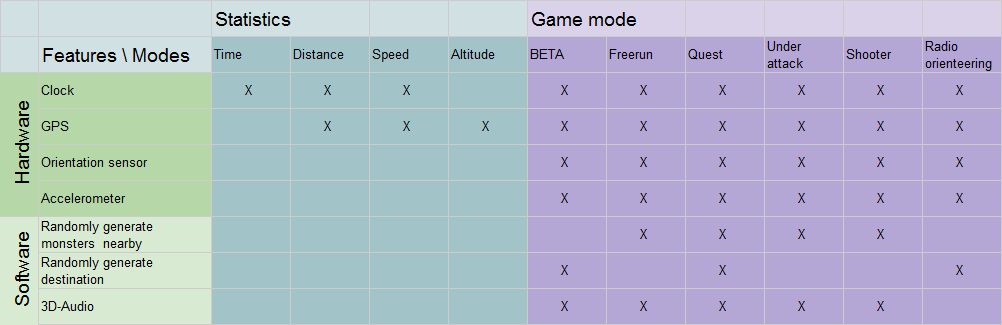
\includegraphics[width=1\textwidth]{tabbellfeatures}\caption{Scheme of what features are needed for different modes\label{fig:Scheme-of-features}}
\end{figure}


\item Evaluation of the BETA concerning usability:

\begin{itemize}
\item By doing testing with actual people the app will be improved on usability.
This will be done in the following steps:

\begin{itemize}
\item Establishing requirements by conducting interviews with test persons
after they have performed certain tasks in the app
\item Designing and prototyping alternatives fitting the requirements
\item Implementing the new design
\end{itemize}
\end{itemize}
\item Finally, if there is time, some advanced and further game functions
will be implemented:

\begin{itemize}
\item Multiplayer - Run together with a friend in the same game-world with
the same coins, monsters and destinations.
\item Game mode including Geocaching%
\footnote{An outdoor ``Treasure hunt'' using GPS \citep{Groundspeak2014}.
\href{http://www.geocaching.com/}{http://www.geocaching.com/}%
} or Geocaching coordinates.
\end{itemize}
\end{enumerate}

\subsection{Plan B - Radio orienteering}

If the initial idea of a using panoration of audio to indicate the
direction of the sound is not accurate enough to make it possible
for the user to find a sound source, the already written code will
be used to make an application to emulate radio orienteering%
\footnote{A sport where the competitors have to find hidden controls by listening
to a signal caught up by a receiver carried by each contestant \citep{Radio-orienteringSverige2014}.%
}.

Instead of real controls and receivers, this application will rely
on generated GPS coordinartes and audio. By turning around with the
phone in hand, the audio level will change depending on if there’s
a control in the direction of which the phone is pointing. To clarify:
no panoration will be involved - just the volume of the audio changing
as the user is rotating (depending on direction to source).

The GPS part of a radio orienteering application would work similar
to how it’d work in our initial application idea. The most drastic
change would be the audio not being panned, but instead relying completely
on the level of the sound always being in the centre - making it an
easier task to get working well. That would eliminate the problems
occurring when trying to make a sound appearing from a certain direction.


\section{Limitations}

The device sensors will limit how accurately the user orientation
can be measured, thereby limiting the user experience.

When starting writing this report, possibilities to enhance the experience
with 3D positional audio was still being researched by members of
the group. There’s an API called OpenSL ES that claims to make it
easy to position audio binaurally (as well as processing it in other
ways) \citep*{KhronosGroup2014}. However, as for 2012, no actual
Android device seemed to support that specific feature \citep{Ratabouil2012}.
Neither did any of the project groups own phones. It turned out a
device had to implement a profile provided by OpenSL ES in order to
make use of all its functions.

Instead, if the sound is supposed to be heard from behind the user,
it will instead appear from one of the ears and gradually move towards
the center as the user is rotating towards the source. A voice or
sound informing the user that he/she is heading towards the wrong
direction might be a good alternative if the former turns out to be
difficult.

When developing the application the assumption that people might listen
to music when running will be considered. Ideally the user should
be able to listen to music while using the application. Alternatively
the experience could perhaps be made fun enough for the user not wanting
to listen to music while using the application.


\section{Method}

Initially, information will be gathered on how to use the Android
APIs in the most efficient way for this kind of application. This
will include how to use activities, sensors and maps. Since the application
is developed to be run entirely on Android platforms, this part of
the research will be of huge importance for the outcome.

Alongside the coding-aspects mentioned above, information will be
gathered on how specific areas (GPS, orientation sensor, audio, etc.)
work and how they’re implemented using Java for Android. Most of the
information will probably come from e-books, as well as Android's
developer pages on the Internet. While doing this research a proof
of concept of the experience of the sound will be made. This proof
of concept will confirm that the sound is sounding as expected in
relation to its location.

When information is gathered the structure of the app will be decided.
Here UML-models will be drawn to make the structure clear. After the
modelling decisions are made sketches will be drawn to decide how
the GUI might look.

Then the coding process will start. The parts to be coded will be
the ones mentioned in \prettyref{sec:Problem/Assignment}. Alongside
with the coding, testing will be made to make sure that everything
is working as expected. When possible, the tests will be made as test
cases. It will also be important to test with real values - such as
going out and running and see how the application works.

An evaluation will be performed when the first BETA-version is finished.
This will be done by letting a test group use our app and conducting
interviews with the test persons. These findings will help us establish
requirements to come up with new design alternatives which later can
be implemented.


\subsection{Development}

The Scrum method will be used when developing the application - a
flexible Agile software development framework where the team works
more as a unit opposed to a traditional and sequential approach. The
division of labor will be done in cycles (sprints). Each job occasion
will begin with a scrum meeting - a short meeting where the group
talks about what’s going on, what’s about to happen as well as possible
problems.

To handle the coding part of the development, Git will be used, which
is a version handling system that makes it easy to collaborate with
others in coding projects. It makes it possible for each team member
to work in the same classes and merge them when needed. Each specific
part of the application (audio, gps etc.) will be implemented in individual
branches.

When it comes to the testing part of the development, both the virtual
phone available in the Android developing environment will be used,
as well as our own phones.


\subsection{Literature studies}

The literature studies will involve how the human ear perceives sound,
and how it’s possible to imitate sounds coming from specific directions
using stereo headphones \citep{Roads1996}.

Literature about Android and how to best develop the app will also
be studied. This is necessary to make the app enjoyable for the user
and flexible enough to work on different kinds of phones. According
to the Android API Guide - Fragments \citeyearpar{AndroidDevelopers2014b},
fragments can decompose the functionality of an app into smaller parts
(fragments) that can be reusable and, depending on the screen size,
show up in different quantities at a time.

Alongside the audio and Android studies, the sensors considering position
and orientation need to be studied. While GPS is the most natural
way to measure the position \citep{Sood2012}, there are various ways
to measure the user orientation. 

The orientation while in motion could be decided through the GPS bearing
\citet*{AndroidDevelopers2014c}, which is calculated as the direction
the phone is travelling in. Although, while standing still and only
rotating on the spot, we might be able to use the magnetic field sensor
(compass) and accelerometer to provide an orientation of the phone
itself \citep{Sood2012}. This however has problems since the orientation
of the phone relative to the actual user is not always known (it depends
on how the user is holding the phone).

Probably, as some initial testing shows, some combination of both
is preferable.


\section{Timetable}

In order to create a preliminary time plan of the important phases
of the project a Gantt chart was used. It is to be found in \prettyref{fig:Gantt Chart}.

\begin{sidewaysfigure}
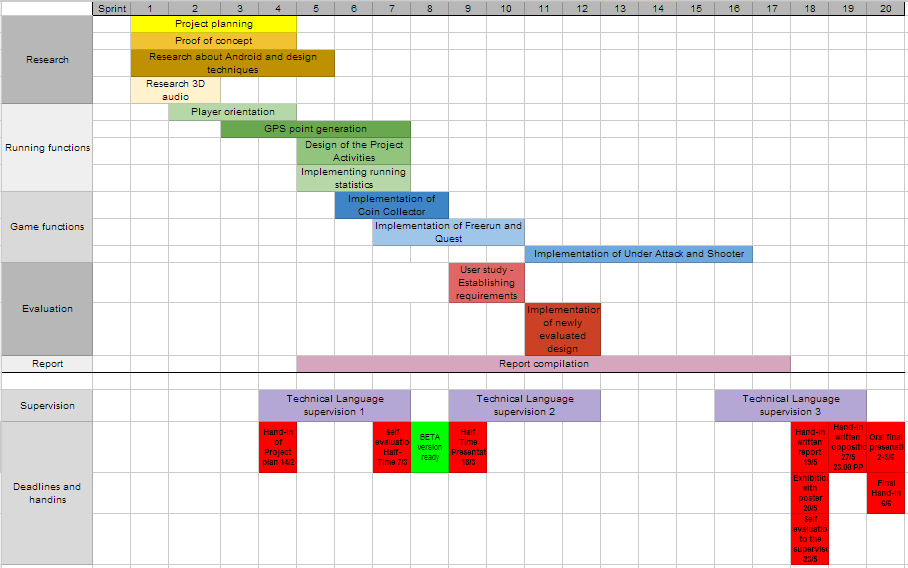
\includegraphics[width=0.9\paperwidth]{timetable}\caption{Preliminary Time Plan for the project \label{fig:Gantt Chart}}
\end{sidewaysfigure}


\pagebreak{}\bibliographystyle{elsarticle-harv}
\phantomsection\addcontentsline{toc}{section}{\refname}\bibliography{References}

\end{document}
